%\providecommand{\main}{..}
%\documentclass[\main/main.tex]{subfiles}


\begin{document}

\section{Constructing the P matrix}




\subsection{Estimates of mortality from SHARE}

In order to compute the mortality risk for SHARE participants, we first fit a Bayesian hierarchical model as specified in section \ref{hierarchical_model}. We are going to perform partial pooling on individuals' histories in our panel dataset. As a second step, we are going to fit a simple logistic regression and compare the two model specifications.\\



The age-specific transition probabilities are estimated for the two possible outcomes (dead or alive), conditional on three covariates only: age, gender and income decile.
Other covariates such as education are not included in the analysis. \\
We do not assume these variables to be uncorrelated to health outcomes, which would probably be a strong and reasonably incorrect assumption. Conversely, the rationale behind this choice is that our focus is on the correlation between income and healthy life expectancy and not on the causal effect. Thus, it does not matter whether other covariates play an important role in explaining the differences in mortality rates, which they reasonably do, as the central focus is at a \lq\lq descriptive'' level.\\


Indeed, from the point of view of policy makers, pension funds, and insurance companies, it might be important to assess a positive correlation between income and life expectancy (both healthy and unhealthy), regardless of driving force of the phenomenon. For instance, no matter the underlying cause, it would still be true that lower-income people have shorter lives and receive government benefits for fewer years in old age, thus reducing the  redistributive role of the pension system. This is, for instance, what \cite{Auerbach2017} show for the American case.\\

Finally, from an operational point of view, any additional regressor would imply a further partition of the dataset when constructing the population matrix for projection. This would make the analysis cumbersome and the results more difficult to interpret. \\

As for the choice of the three regressors, the first one (i.e. age) is necessary in order to obtain survival and mortality probabilities for each age group, the second (i.e. income) is our focal variable, and the third one (i.e. gender) is added since it is well-documented that female tend to live longer than men. See, for instance, the research by \cite{Austad2006WhyLongevity} exploring sex differences in longevity. Moreover, retirement age typically differ by gender and therefore it might be useful to reason about these two categories separately from a policy perspective.\\

In order to obtain the posterior distribution of the set of parameters, we exploit as sampling method as outlined in section \ref{sampling_method}. \\
There are different software packages that allow to sample posterior distributions using MCMC methods. Our choice was to use the python package pySTAN, which is based upon the STAN probabilistic language.\\

Below we present the full model written in STAN:
\\

\begin{lstlisting}[language=Python]
data {
    int N;                      // Number of rows
    int K;                      // Number of individuals
    int<lower=0, upper=1> y[N]; // Observed outcome vector
    int M[N];                   // Mapping of rows to individual history
    real age[N];                // Observed individual ages
    real income[N];             // Observed individual incomes
    real gender[N];             // Observed individual genders
}
parameters {
    real common_age;
    real common_income;
    real common_gender;

    real common_sigma_age;
    real common_sigma_income;
    real common_sigma_gender;

    real alpha;
    real beta_age[K];
    real beta_income[K];
    real beta_gender[K];

    real sigma_age;
    real sigma_income;
    real sigma_gender;
}
model {
    common_sigma_age ~ uniform(0, 20);
    common_sigma_income ~ uniform(0, 20);
    common_sigma_gender ~ uniform(0, 20);

    sigma_age ~ uniform(0, 20);
    sigma_income ~ uniform(0, 20);
    sigma_gender ~ uniform(0, 20);

    common_age ~ normal(0, common_sigma_age);
    common_income ~ normal(0, common_sigma_income);
    common_gender ~ normal(0, common_sigma_gender);

    alpha ~ normal(0, 20);
    beta_age ~ normal(common_age, sigma_age);
    beta_income ~ normal(common_income, sigma_income);
    beta_gender ~ normal(common_gender, sigma_gender);

    for(i in 1:N) {
        y[i] ~ bernoulli(
            inv_logit( // Softmax
                alpha + beta_age[M[i]] * age[i] + beta_income[M[i]] * income[i] + beta_gender[M[i]] * gender[i]
            )
        );
    }
}
\end{lstlisting}
\vspace{1cm}
The second step in the process of estimation of the mortality probabilities consisted in a comparison of the results obtained with the above model to those obtained by a simple pooled logistic regression. As we can see from the figures below, the median of the posterior distribution of the coefficients and the estimated coefficients from the pooled logistic regression are comparable. We show the result for Germany but the same holds true for all the countries in our sample.\\


Therefore, given that the Bayesian hierarchical model takes roughly 30 minutes per country to run, we eventually decided to run the rest of the analysis using the coefficients obtained from the simple pooled logistic model. Our choice is motivated by simple computational efficiency reasons. Nevertheless, the importance of having run this comparison is crucial as it allowed us to confirm that we are using a simpler model which is, however, robust even if it doesn't take into consideration the panel dimension of the dataset.\\

\begin{figure}[H]
\centering
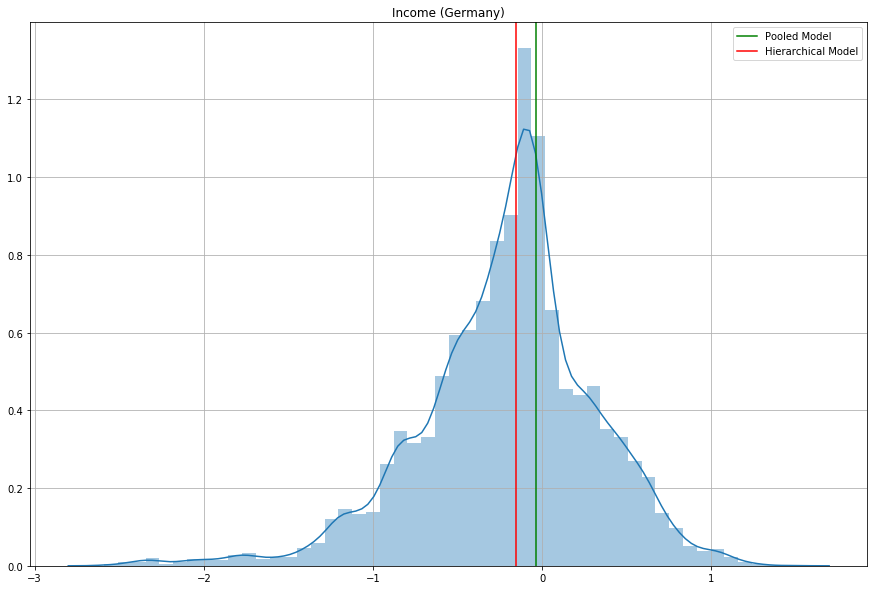
\includegraphics[scale=.3]{images/bayesian/download-36.png}
            \captionsetup{justification=centering}
    \caption{Posterior distribution for income coefficient \\
    \textit{Source:} re-produced from EASYSHARE}
    \label{fig:age_distr_germany}
\end{figure}


\begin{figure}[H]
\centering
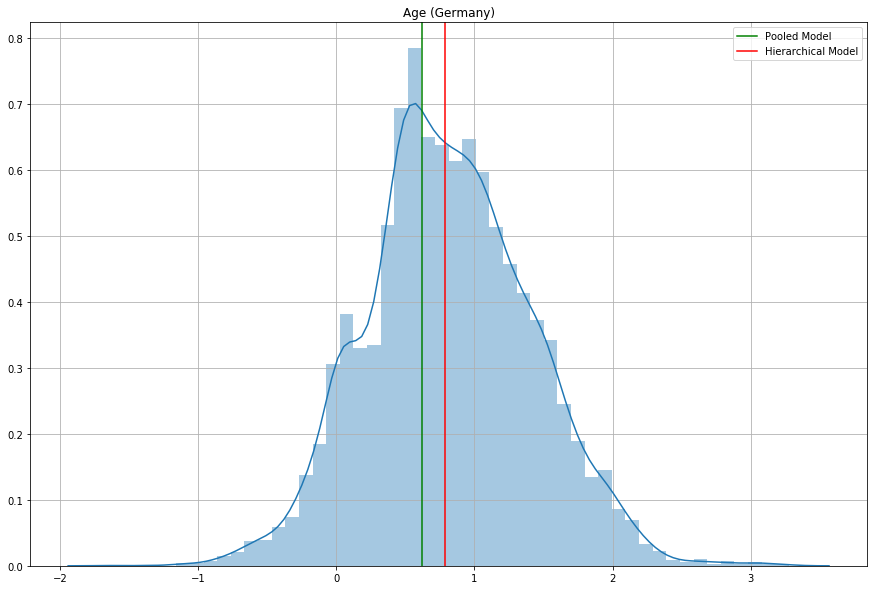
\includegraphics[scale=.3]{images/bayesian/download-37.png}
            \captionsetup{justification=centering}
    \caption{Posterior distribution for age coefficient \\
    \textit{Source:} re-produced from EASYSHARE}
    \label{fig:age_distr_germany}
\end{figure}

\begin{figure}[H]
\centering
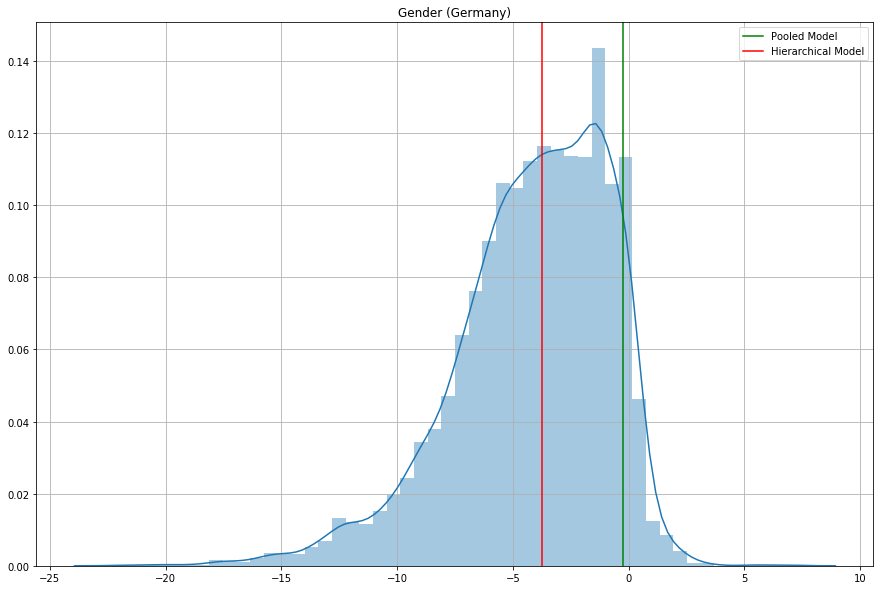
\includegraphics[scale=.3]{images/bayesian/download-38.png}
            \captionsetup{justification=centering}
    \caption{Posterior distribution for gender coefficient \\
    \textit{Source:} re-produced from EASYSHARE}
    \label{fig:age_distr_germany}
\end{figure}


\subsection{Estimates of mortality from HMD}\label{HMD}

We are going to construct an average of the probability of death from the HMD that should at best compare to the estimates from SHARE. The method we followed is briefly outlined below.\\

First of all, we downloaded from the HMD website the period life tables for our nine selected countries. A period life table represents the hypothetical experience of a synthetic cohort, i.e. a cohort that follows the age-specific death rates of a given period. These rates can be computed by looking at the mortality experience of all cohorts who are present during the period and then by \lq\lq hypothetically'' applying them to the synthetic cohort.\\
In other words, the life tables from the HMD describe the distribution of the time it takes the synthetic cohort of individuals to experience the \lq\lq death'' event. The HMD describes this distribution for each separate year. In particular, we are considering the value of
$q_x$ in the life table, i.e. the probability of dying between (exact) age $x$ and (exact) age $x+1$. \\

As a second step, we selected only those years corresponding to the years of interviews in SHARE, namely 2004, 2005,  2006, 2007, 2009, 2010, 2011, 2012, 2013. Figure \ref{dying_female} and \ref{dying_male} show the probability of dying from one year to the next, starting from age 50 up to age 90, for female and male population respectively, as retrieved from the HMD life tables. As expected, the mortality risk has not changed much over the ten-year time horizon we are considering.


\begin{figure}[H]
\centering \textbf{Female population}\par\medskip
\minipage{0.32\textwidth}
  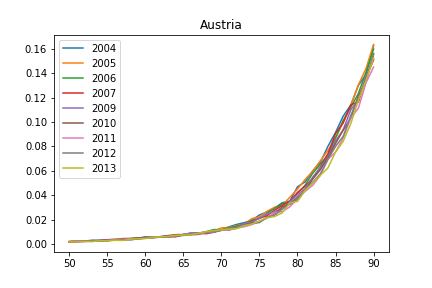
\includegraphics[width=\linewidth]{images/mortality_female_1.png}
\endminipage\hfill
\minipage{0.32\textwidth}
  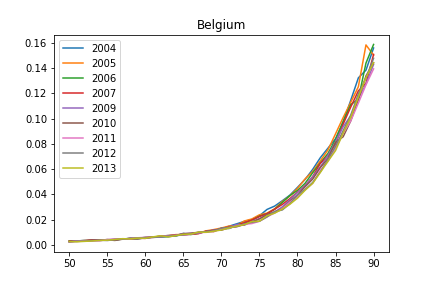
\includegraphics[width=\linewidth]{images/mortality_female_2.png}
\endminipage\hfill
\minipage{0.32\textwidth}%
  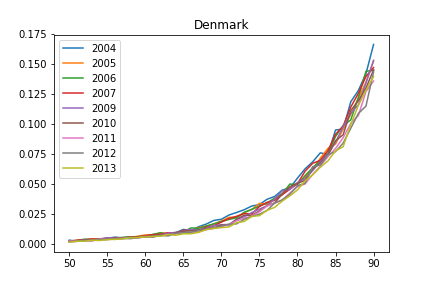
\includegraphics[width=\linewidth]{images/mortality_female_3.png}
\endminipage \hfill
\minipage{0.32\textwidth}
  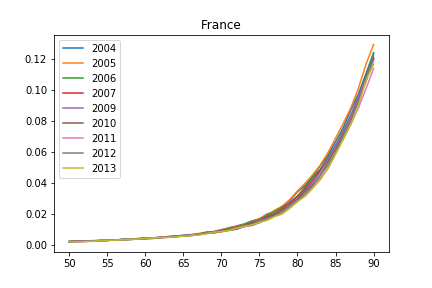
\includegraphics[width=\linewidth]{images/mortality_female_4.png}
\endminipage\hfill
\minipage{0.32\textwidth}
  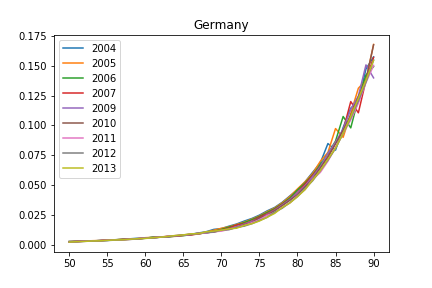
\includegraphics[width=\linewidth]{images/mortality_female_5.png}
\endminipage\hfill
\minipage{0.32\textwidth}%
  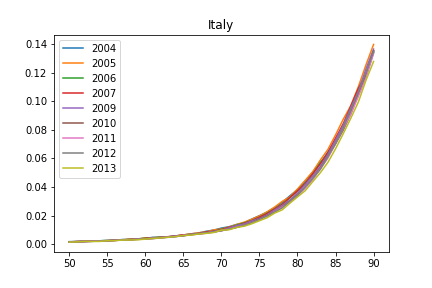
\includegraphics[width=\linewidth]{images/mortality_female_6.png}
\endminipage\hfill
\minipage{0.32\textwidth}
  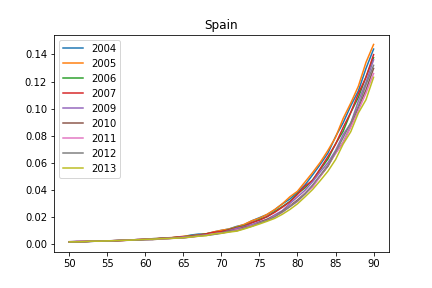
\includegraphics[width=\linewidth]{images/mortality_female_7.png}
\endminipage\hfill
\minipage{0.32\textwidth}
  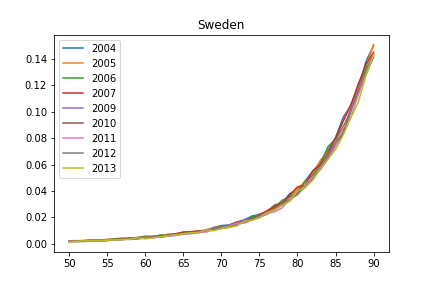
\includegraphics[width=\linewidth]{images/mortality_female_8.png}
\endminipage\hfill
\minipage{0.32\textwidth}%
  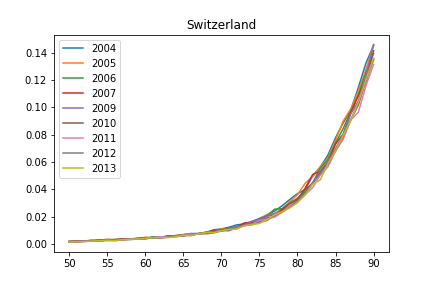
\includegraphics[width=\linewidth]{images/mortality_female_9.png}
\endminipage\hfill
\captionsetup{justification=centering}
\caption{Probability of dying from age $x$ to $x+1$ in 9 different years by country.\\ \textit{Source:} re-produced from the Human Mortality Database}
\label{dying_female}
\end{figure}



\begin{figure}[H]
\centering \textbf{Male population}\par\medskip
\minipage{0.32\textwidth}
  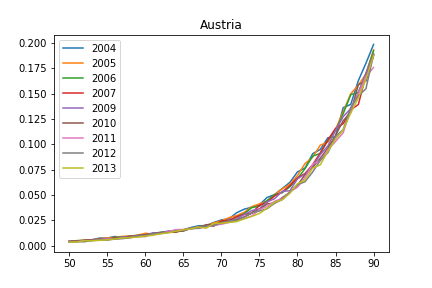
\includegraphics[width=\linewidth]{images/mortality_male_1.png}
\endminipage\hfill
\minipage{0.32\textwidth}
  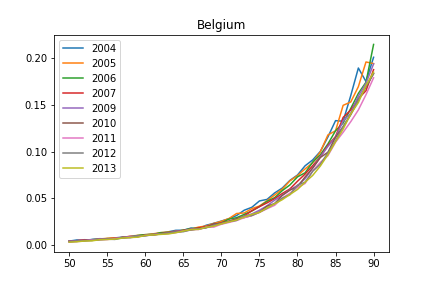
\includegraphics[width=\linewidth]{images/mortality_male_2.png}
\endminipage\hfill
\minipage{0.32\textwidth}%
  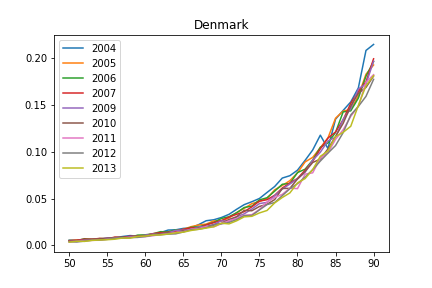
\includegraphics[width=\linewidth]{images/mortality_male_3.png}
\endminipage \hfill
\minipage{0.32\textwidth}
  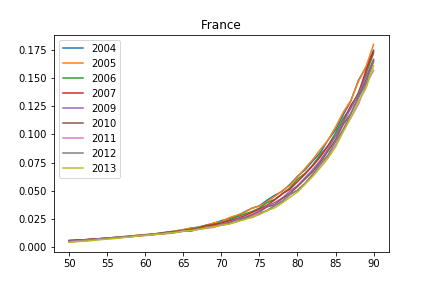
\includegraphics[width=\linewidth]{images/mortality_male_4.png}
\endminipage\hfill
\minipage{0.32\textwidth}
  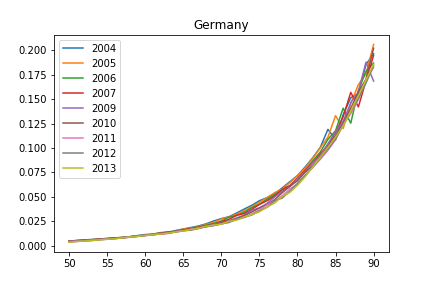
\includegraphics[width=\linewidth]{images/mortality_male_5.png}
\endminipage\hfill
\minipage{0.32\textwidth}%
  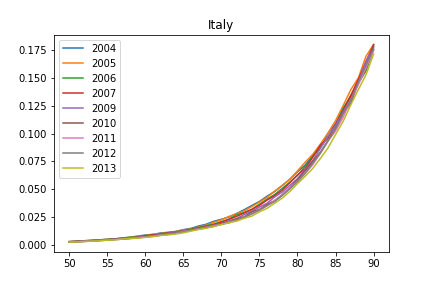
\includegraphics[width=\linewidth]{images/mortality_male_6.png}
\endminipage\hfill
\minipage{0.32\textwidth}
  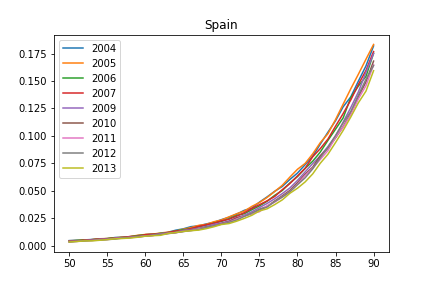
\includegraphics[width=\linewidth]{images/mortality_male_7.png}
\endminipage\hfill
\minipage{0.32\textwidth}
  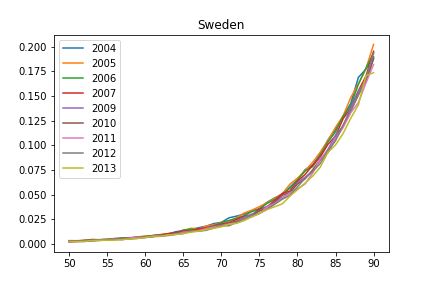
\includegraphics[width=\linewidth]{images/mortality_male_8.png}
\endminipage\hfill
\minipage{0.32\textwidth}%
  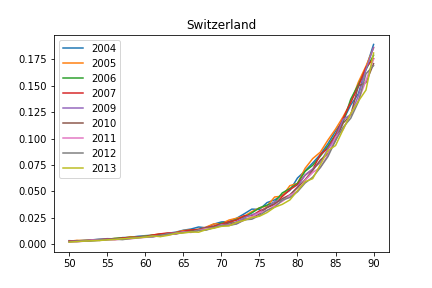
\includegraphics[width=\linewidth]{images/mortality_male_9.png}
\endminipage\hfill
    \captionsetup{justification=centering}
\caption{Probability of dying from age $x$ to $x+1$ in 9 different years by country\\ \textit{Source:} re-produced from the Human Mortality Database}
\label{dying_male}
\end{figure}



Given the little variation over time, as third step, we compute an average of the mortality risk for all ages and countries.
For instance, the probability of dying from age 50 to age 51 in Austria will be computed by summing up all the death risk at age 50 and then dividing by the number of years considered. Figure \ref{fig:averages_0} represents these averaged probability for the female and male population, respectively. \\



\begin{figure}[H]
    \centering \textbf{Average mortality risk by country}\par\medskip
    \begin{minipage}{.5\textwidth}
        \centering
        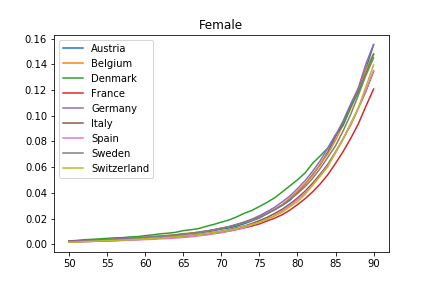
\includegraphics[scale=.5]{images/Average_mortality_female.png}
    \end{minipage}%
   \begin{minipage}{.5\textwidth}
        \centering
       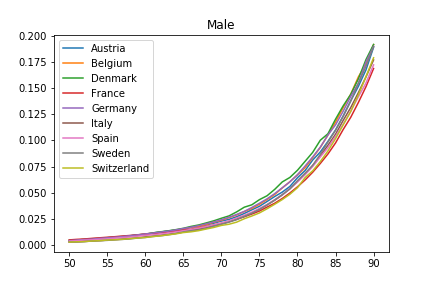
\includegraphics[scale=.5]{images/Average_mortality_male.png}
    \end{minipage}
      \captionsetup{justification=centering}
    \caption{Average probability of dying from age $x$ to $x+1$   over 9 years by country \\ \textit{Source:} re-produced from the Human Mortality Database }
    \label{fig:averages_0}
\end{figure}

As fourth step, we computed an average over all countries to obtain a \lq\lq single'' mortality regime.   

\begin{figure}[H]
    \centering \textbf{Average mortality risk}\par\medskip
        \centering
        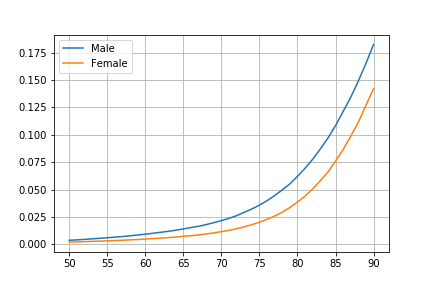
\includegraphics[scale=.5]{images/Average_mortality_all_countries.png}
          \captionsetup{justification=centering}
    \caption{Average probability of dying from age $x$ to $x+1$   over 9 years, all countries. \\ \textit{Source:} re-produced from the Human Mortality Database }
    \label{fig:averages_1}
\end{figure}

A first remark is that this mortality regime is a synthetic measure that aggregates data from different countries, and, as such, it is inevitably introducing some bias. \\
A second remark is that respondents in SHARE were also interviewed in the year 2015. However, the HMD provides information on mortality data only up to 2013 for some countries, e.g. Austria, Italy, and Spain.\\
We decided to exclude the data from 2015 of the HMD for all countries, in order to avoid counting an extra observation for those nations presenting data up to 2015 compared to the ones missing this information.\\
Again, this will introduce some inaccuracy, as we are comparing the mortality regime of two slightly different time horizons (from 2004 to 2013 in the case of HMD and from 2004 to 2015 for SHARE data). 



\subsection{Comparison between mortality risk estimated from SHARE and HMD}
In order to evaluate the estimated mortality risk we computed from SHARE, we plot the probability of dying from one year to the next against the average values obtained from the HMD. We take again Germany as a representative example, considering the estimated probability of dying for individuals in income decile 5.\\

\begin{figure}[H]
    \centering 
\minipage{0.48\textwidth}
\centering \textbf{SHARE}\par\medskip
  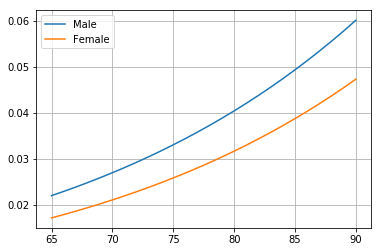
\includegraphics[width=\linewidth]{images/germany_SHARE.png}
 \endminipage\hfill
\minipage{0.48\textwidth}
\centering \textbf{HMD}\par\medskip
  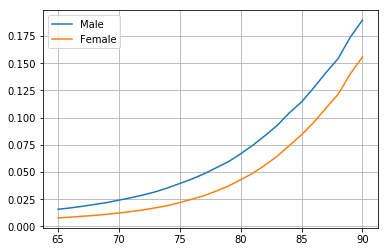
\includegraphics[width=\linewidth]{images/germany.png}
\endminipage\hfill
        \captionsetup{justification=centering}
    \caption{Average probability of dying from age $x$ to $x+1$ in Germany. \\
    \textit{Source:} re-produced from SHARE and the Human Mortality Database }
    \label{fig:averages_2}
\end{figure}


By looking at the graph, it is clear that we are underestimating mortality risk, especially at old ages. This is an important aspect that will affect the computation of life-expectancy as well. Therefore, when interpreting the main output of interest of this research, one should consider that we are probably estimating a \lq\lq higher '' life-expectancy than the one we could probably observe if we were to run the analysis on other datasets.


\end{document}